\chapter{Graph pattern definition in \viatra{} query language (VQL)}
\label{chapter:vql}

Graph patterns can be defined using \viatra{} Query Language (VQL). 
The language syntax is simple, although complex queries are not always self evident how to be expressed.

\section{ Language Constructs }

\subsection{Pattern definition}
Patterns and its bodies can be given by the \emph{pattern} keyword. 
Parameters must be specified after the parameter name in round brackets. 
Bodies of the pattern are given in curly brackets, separated by the \texttt{or} keyword

\begin{minipage}{\textwidth}
\begin{lstlisting}[language=vql]
pattern patternName( p1: Type1, p2: Type2){
... // Constraints for first body
} or {
... // Constraints for second body
} ...
\end{lstlisting}
\end{minipage}


\subsection{Constraints}
Constraints are given like statements. 
Each constraint is followed by a semicolon.

\vspace{\abovedisplayskip}
\begin{minipage}{\textwidth}
Type constraint can be given by specifying the type, then the object in round brackets.
\begin{lstlisting}[language=vql]
pattern patternName( o ){
	Type(o);
}
\end{lstlisting}
\end{minipage}
\vspace{\belowdisplayskip}

\begin{minipage}{\textwidth}
Reference constraint can be given by specifying which type's which reference must be checked, then giving the source and target variables in round brackets:
\begin{lstlisting}[language=vql]
pattern patternName( p1: Person, p2: Person ){
	Person.friend(p1, p2);
}
\end{lstlisting}
\end{minipage}
\vspace{\belowdisplayskip}

\begin{minipage}{\textwidth}
Other patterns can be used as constraint with the \texttt{find} keyword:
\begin{lstlisting}[language=vql]
pattern patternName( p1: Type1, p2: Type2, p3: Type3 ){
	find otherPatternName(p1, p2);
	find otherPatternName(p2, p3);
}
\end{lstlisting}

Also we can use underscore instead of specifying parameters. 
This way the constraint is satisfied, if the pattern matches with anything in the place of underscores (existential quantification).
\begin{lstlisting}[language=vql]
pattern patternName( p1: Type1 ){
find otherPatternName(p1, _);
}
\end{lstlisting}

This is the same as the following (if x is not used anywhere else):
\begin{lstlisting}[language=vql]
pattern patternName( p1: Type1 ){
find otherPatternName(p1, x);
}
\end{lstlisting}
\end{minipage}
\vspace{\belowdisplayskip}

\begin{minipage}{\textwidth}
negative pattern match can be expressed by \texttt{neg find} keyword:
\begin{lstlisting}[language=vql]
pattern patternName( p1: Type1, p2: Type2 ){
	neg find otherPattern(p1, p2);
	Type1.reference(p1, p2);
}
\end{lstlisting}

Also, we can use underscore if we don't want that the other pattern match occurs with \emph{any} value at the underscores. ( ie.\ \texttt{neg find} can be used to express negated existential quantification along with negated expressions )

\begin{lstlisting}[language=vql]
pattern patternName( p1: Type1 ){
	neg find otherPattern(p1, _);
}
\end{lstlisting}

It is very important to clarify, that unlike in the case of find this is \emph{not} the same as the following:

\begin{lstlisting}[language=vql]
pattern patternName( p1: Type1 ){
	neg find otherPattern(p1, x);
}
\end{lstlisting}
As this will match if there exist \emph{any} x, that (p1, x) not satisfies the \texttt{otherPattern}.


\end{minipage}
\vspace{\belowdisplayskip}



\begin{minipage}{\textwidth}
\texttt{count find} can be used to count maches to a given pattern (Counting the ways underscores can be bound to form a match for the other pattern)
\begin{lstlisting}[language=vql]
pattern personPattern(p){
	Person(p)
}

pattern countPersons(cnt)
	cnt == count find personPattern(_);
}
\end{lstlisting}
	
\end{minipage}
\vspace{\belowdisplayskip}



\begin{minipage}{\textwidth}
Equality and inequality also can be given between variables ( ==, != ):
\begin{lstlisting}[language=vql]
pattern friendsOfFriends(a, b){
	Person.friend(a, x);
	Person.friend(x, b);
	a != b;
}

pattern sameOrFriend(a : Person, b: Person){
	Person.friend(a, b);
} or {
	a == b;
}
\end{lstlisting}
	
Equality constraint is mostly used between parameters, as in other cases simply using one variable instead of using two and making them equal is simpler.  
	
\end{minipage}
\vspace{\belowdisplayskip}



\begin{minipage}{\textwidth}
The keyword \texttt{check} can be used to create a constraint, that a given java (XBase) expression is true. The expression only can refer to attribute  variables (Variables refering to data types instead of graph nodes).
\begin{lstlisting}[language=vql]
pattern adultPerson( p: Person ){
	Person.age(p, age);
	check(age >= 18);
}
\end{lstlisting}
\end{minipage}
\vspace{\belowdisplayskip}

\begin{minipage}{\textwidth}
The keyword \texttt{eval} can be used to evaluate a java (XBase) expression on attribute variables and assign the result to another variable.
\begin{lstlisting}[language=vql]
pattern patternName( p1: Person, p2: Person, agesum : EInt ){
	Person.age(P1, a1);
	Person.age(P2, a2);
	agesum == eval(a1 + a2);
}
\end{lstlisting}
\end{minipage}
\vspace{\belowdisplayskip}

\subsection{Annotations}

\begin{minipage}{\textwidth}
Annotations can be added to patterns with the following syntax:
\begin{lstlisting}[language=vql]
@AnnotationName(
	a = {p1, p3}
	a = {p2, p3}
	b = "A simple string"
)
@AnnotationName2
pattern patternName( p1, p2, p3, ... )
	...
\end{lstlisting}
\end{minipage}
\vspace{\belowdisplayskip}

An annotation has a name (after \texttt{@}), and some named attributes using \texttt{name = value} syntax in parentheses.
One attribute name can be used multiple times. 
The attribute's value can be a single value or a list of values, that can be strings, numerals, or parameter reference.


\subsubsection{Annotations used by our framework}

The framework processes the following two types of annotations:
\begin{itemize}
	\item \texttt{@Bind} can be used to control what kind of graph pattern matching code will be generated, ie.\ what parameter sets can be bind to restrict the results. The version of the query, where all the parameters are unbound is generated by default.
	
	\item \texttt{@SkipDefaultGen} can be used to avoid default query generation for unbound version, eg.\ in case of helper patterns, we would not want to use it by itself most of the time.
	
\end{itemize}


\section{VQL examples from the case study}
\label{sec:vql-examples}

To show how these elements can be used in patterns, now we present the benchmarked queries, and what their semantics are, for this we show, what subgraphs these patterns matches from the graph depicted in \autoref{fig:query-example-model}. This simple model represents 3 sequences of railroad elements and a Turnout (7) between them. \texttt{connectedTo} references are symmetrical.
\vspace{0.1\textwidth}


\begin{figure}[H]
	\begin{center}
		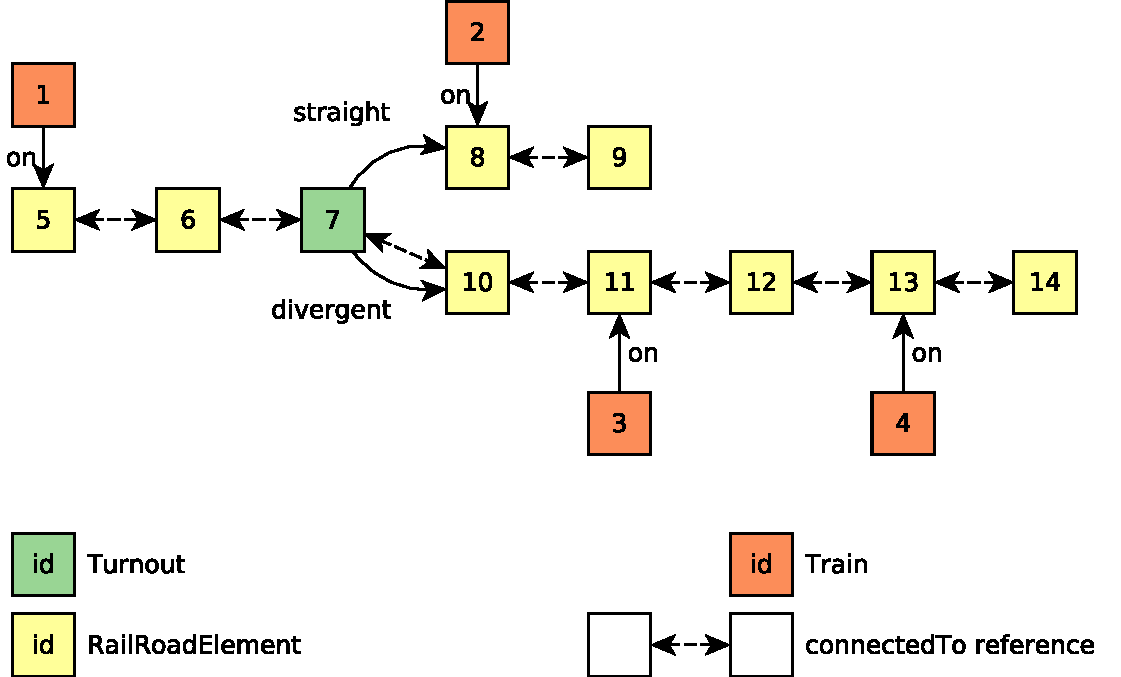
\includegraphics[width=\textwidth]{figures/query-example-model.pdf}
		\caption{Example model}
		\label{fig:query-example-model}
	\end{center}
\end{figure}

\subsection{\texttt{trainLocations}}
\begin{minipage}{\textwidth}

\texttt{trainLocations} pattern matches for all the (\texttt{train},\texttt{loc}) pairs where \texttt{train} is a Train, that is on the location \texttt{loc}.
Using this pattern we can query all the trains, and where they are.
As \texttt{@Bind} annotation denotes, we can also bind the train parameter: this way we can query where a specific train is.
\begin{lstlisting}[language = vql]
@Bind( parameters=train )
pattern trainLocations(train: Train, loc: RailRoadElement)
{
	Train.on(train, loc);
}
\end{lstlisting}
We can see the matches of the pattern in \autoref{fig:match-trainLocations}. The matches are the train-location pairs with \texttt{id}s (1,5), (2,8), (3,11) and (4,13).
\begin{figure}[H]
	\begin{center}
		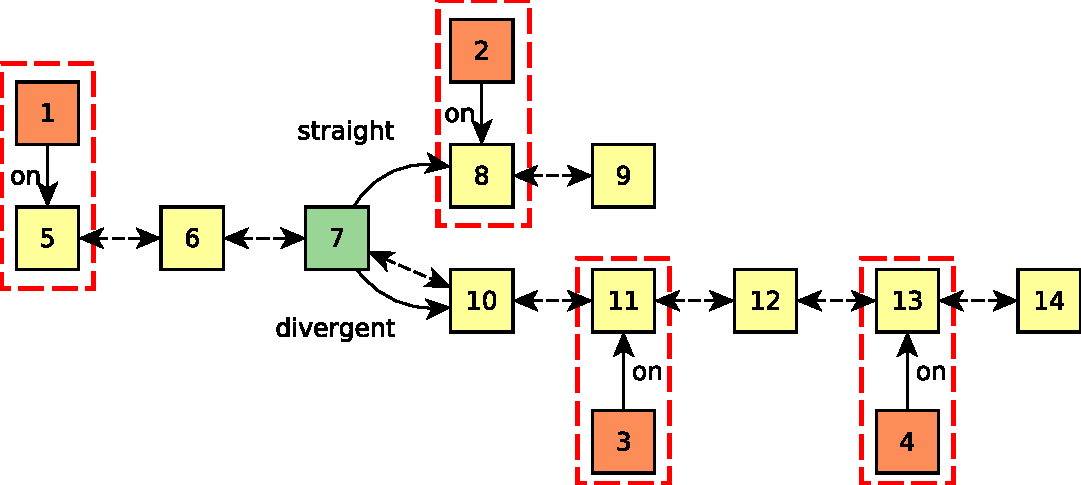
\includegraphics[width=0.8\textwidth]{figures/query-example-model-trainloc.pdf}
	\end{center}
	\caption{Matches of the \texttt{trainLocations} pattern}
	\label{fig:match-trainLocations}
\end{figure}

\end{minipage}


\subsection{\texttt{endOfSiding}}

End of siding pattern matches, when there is a last segment of railroad, and a train is near to that segment.
The last segment is expressed as a \texttt{RailRoadElement}, which has a neighbor, but only one.
If a train is on the neighbor, the pattern matches.
We use the annotation \texttt{@SkipDefaulGen} on the \texttt{connected} pattern, because it is only needed as a subpattern.

\begin{minipage}{\textwidth}
\begin{lstlisting}[language = vql]
pattern endOfSiding(train: Train, end: RailRoadElement, neighbor: RailRoadElement)
{
	RailRoadElement.train(neighbor, train);		
	RailRoadElement.connectedTo(end,neighbor);
	1 == count find connected(end,_);	
}

@SkipDefaultGen
private pattern connected(a : RailRoadElement, b : RailRoadElement){
	RailRoadElement.connectedTo(a,b);
}
\end{lstlisting}

\end{minipage}

We can see the matches of the pattern in \autoref{fig:match-endOfSiding}. 
The matches are the train-end-neighbor tuples with \texttt{id}s (2,9,8) and (4,14,13). 
We can see, that both of the \texttt{RailRoadElement} with id=9 and the \texttt{RailRoadElement} with id=14 has only one \texttt{connectedTo} reference, and their only neighbors have trains on them.

\begin{figure}[H]
	\begin{center}
		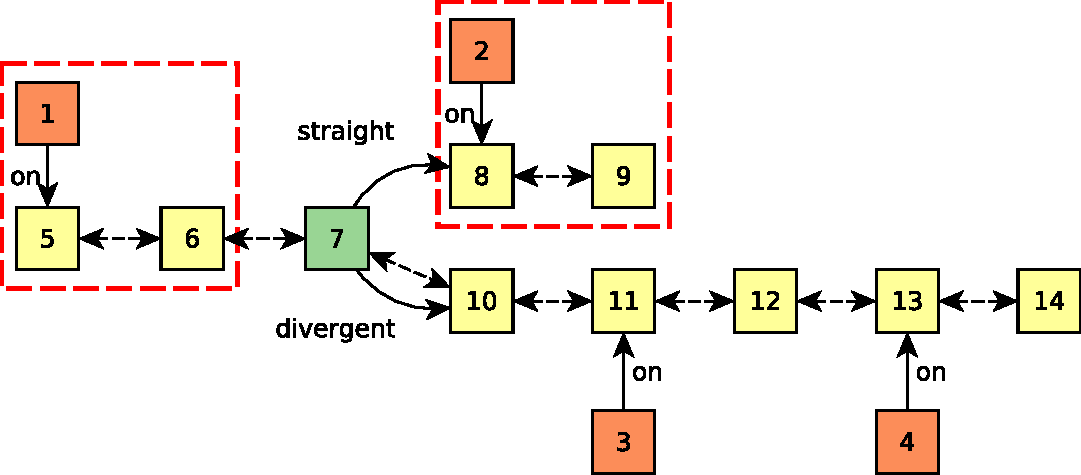
\includegraphics[width=0.8\textwidth]{figures/query-example-model-endofsiding.pdf}
	\end{center}
	\caption{Matches of the \texttt{endOfSiding} pattern}
	\label{fig:match-endOfSiding}
\end{figure}



\subsection{\texttt{derailment}}
\begin{minipage}{\textwidth}
	
\texttt{derailment} matches, when a train is on the non-connecting side of a turnout:
The turnout switches between the straight and the divergent railroad. 
connectedTo reference points to the selected segment and the third, always connecting segment.
So if a train is on a straight or the divergent segment (1, 2), but that segment does not connected to the turnout(3), then the pattern matches to this train-segment pair.


\begin{lstlisting}[language = vql]
pattern derailment(elem: RailRoadElement, train: Train)
{
	Turnout(turnout);
	RailRoadElement.train(elem,train); 		// (1)
	find straightOrDivergent(turnout, elem) // (2)
	neg find connected(elem, turnout); 		// (3)
}

@SkipDefaultGen
private pattern straightOrDivergent(turnout : Turnout, elem : RailRoadElement){
	Turnout.straight(turnout, elem);
} or {
	Turnout.divergent(turnout, elem);
}

@SkipDefaultGen
private pattern connected(a : RailRoadElement, b : RailRoadElement){
	RailRoadElement.connectedTo(a,b);
}

\end{lstlisting}
\end{minipage}

We can see the match of this pattern in \autoref{fig:match-derailment}. 
the \texttt{Turnout} with id=7 has a straight side \texttt{RailRoadElement} with id=8 and a \texttt{Train} with id=2 on it. However, this segment is not connected to the turnout, which means, that the turnout is switched to its divergent side.
This is the condition which causes the pattern to match on the \texttt{Train}-\texttt{RailRoadElement} pair with \texttt{id}s (2,8).

\begin{figure}[H]
	\begin{center}
		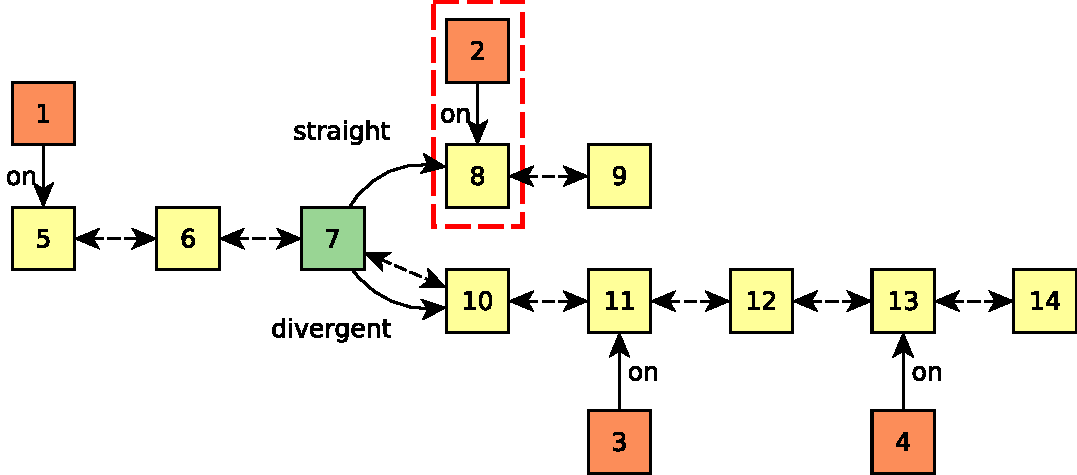
\includegraphics[width=\textwidth]{figures/query-example-model-derailment.pdf}
	\end{center}
	\caption{Match of the \texttt{derailment} pattern}
	\label{fig:match-derailment}
\end{figure}


\vspace{\belowdisplayskip}







\subsection{\texttt{closeTrains}}

Two trains are close, if they are on two segments (start, end) that are connected by another segment (middle). The two train and the two segments are different\footnote{This is important, because it is not mandatory for variables to be different.}.
The result of the pattern is the two segments.

E.g\ in \autoref{fig:match-closeTrains} we can see, that the match of these queries are the \texttt{RailRoadElement} pair with ids (11, 13) and (13, 11). 

Without the inequality constraints there could be matches, like (5, 5), bacause
\begin{itemize}
	\item start = end = (the \texttt{RailRoadElement} with id=5)
	\item t1 = t2 = (the \texttt{train} with id=1)
	\item middle = (the \texttt{RailRoadElement} with id=6)

\end{itemize}
would also satisfy the other constraints.

\begin{minipage}{\textwidth}
\begin{lstlisting}[language = vql]
pattern closeTrains(start : RailRoadElement, end : RailRoadElement)
{
	Train.on(t1,start);
	Train.on(t2, end);
	
	RailRoadElement.connectedTo(start,middle); 
	RailRoadElement.connectedTo(middle, end);
		
	start != end; 
	t1 != t2;	
}
\end{lstlisting}
\end{minipage}

\begin{minipage}{\textwidth}
We can also improve on this query to filter "mirrored" matches:
\begin{lstlisting}[language = vql]
pattern closeTrains(start : RailRoadElement, end : RailRoadElement)
{
	Train.on(t1,start);
	Train.on(t2, end);
	
	RailRoadElement.connectedTo(start,middle); 
	RailRoadElement.connectedTo(middle, end);

	Train.id(t1, id1);
	Train.id(t2, id2);
	check(id1 < id2);
	
}
\end{lstlisting}
In the evaluation of the framework, we used the former version of \texttt{closeTrains}
\end{minipage}

\begin{figure}[H]
	\begin{center}
		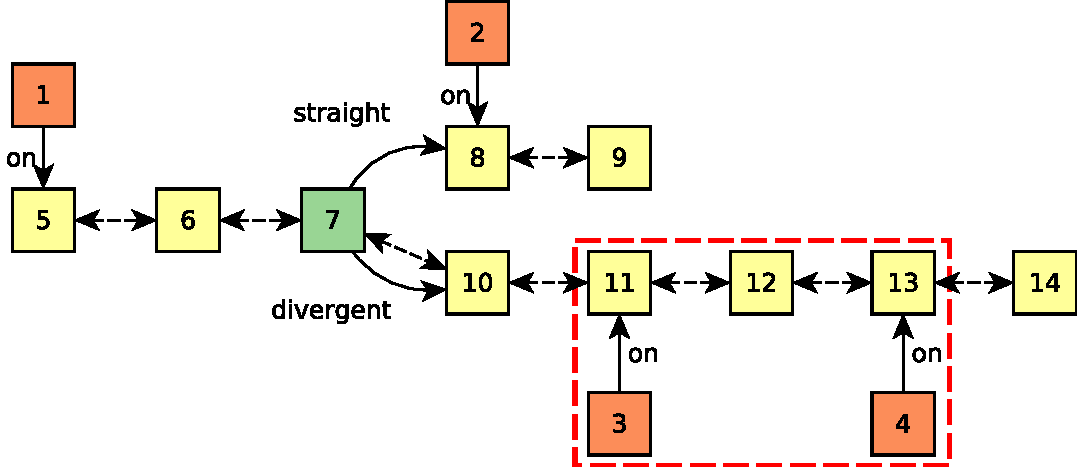
\includegraphics[width=\textwidth]{figures/query-example-model-closetrains.pdf}
	\end{center}
	\caption{subgraph matching the \texttt{closeTrains} pattern}
	\label{fig:match-closeTrains}
\end{figure}









